\documentclass[10pt, serif, mathserif]{beamer}

\usetheme{metropolis}

\usepackage{booktabs}
\usepackage[scale=2]{ccicons}
\usepackage[outputdir=output]{minted}

\usemintedstyle{pastie}

\setmonofont{FiraMono-Regular.ttf}

\title{Random number generation}
\subtitle{Quantitative Risk Management project work}
\date{}
\author{Silvia Baldisserotto, Maysa Jahanbani, \\ Claudia Pesci, Phan Ho Tan Phat, \\ Andrea Venuta}
\institute{Università degli Studi di Firenze - Finance and Risk Management}

\renewcommand{\theFancyVerbLine}{\sffamily \textcolor[rgb]{0.5,0.5,0.5}{\small \oldstylenums{\arabic{FancyVerbLine}}}}

\begin{document}

\maketitle

\begin{frame}
  \frametitle{Random numbers}
  \begin{itemize}
  	\item Computer-generated numbers are \emph{pseudo-random}: \\ deterministic and predictable
  	\item \emph{Quasi-random} numbers prevent potential lack of equidistributedness
  	\item \textbf{Definition.} \emph{(Sample)}. A sequence of number is called a \emph{sample from the distribution $F$}
  	  if the numbers are independent realizations of a random variable with distribution function $F$
	\item Uniform deviates: samples from $\sim \mathcal{U}  \left[ 0, 1 \right] $
	\item Normal deviates: samples from $\sim \mathcal{N}  \left( 0, 1 \right) $
	\item Drawing uniform deviates is the basis of \\ random number generation
  \end{itemize}
\end{frame}

\begin{frame}
  \frametitle{Linear congruential generators}
  	\begin{itemize}
  	  \item $N_0$ is chosen arbitrarily (called the \emph{seed})
  	  \item $N_i = (aN_{i-1} + b)\ \text{mod}\ M$ for $i > 0$, then
  	    \\ \[U_i = \frac{N_i}{M},\quad U_i \in \left[0,1\right)\] 
        \medskip
  	  \item Suitability of the numbers $U_i$ depends on how $a, b, M$ are chosen
  	\end{itemize}
\end{frame}

\begin{frame}
  \frametitle{Linear congruential generators: properties}
  \begin{itemize}
    \item Numbers $N_i$ are periodic, with period $\leq M$: \\ there are at most $M$ different numbers in the class modulo $M$
    \item Examples:
      \begin{itemize}
        \item If $N=0$, $b$ can't be $0$, otherwise $N_i = 0$ will repeat itself
        \item If $a=0$, generator settles down on $N_n = N_0 + nb$
      \end{itemize}
    \item Numbers are distributed ``evenly'' if we have exactly $M$ different numbers in a generator with modulo $M$, or
    \item Each grid point on a \emph{mesh} on $\left[0,1\right]$ with size $\frac{1}{M}$ is occupied once
  \end{itemize}
\end{frame}

\begin{frame}
  \frametitle{Quality of generators}
  Requirements:
  \begin{enumerate}
  	\item Large period: small set of numbers makes the outcome easier to predict (choose M as large as possible)
  	\item Statistical tests to verify that the distribution is the intended one
  	  \begin{itemize}
  	  	\item Comparison of sample mean and variance $\mu,\ \sigma^2$ \\ with desired values
  	  	\item Correlation between sample values
  	  	\item Quality of approximation of the distribution
  	  \end{itemize}
     \item Distribution in higher dimensional spaces: lattice structure
  \end{enumerate}
\end{frame}

\begin{frame}
  \frametitle{Random vectors and lattice structure}
  \begin{itemize}
  	\item Sequences of random numbers can be arranged in \\ $m$-dimensional vectors
  	\item The vectors lie on a number of parallel \\ $(m-1)$-dimensional hyperplanes
  	\item The ideal condition is that the number of parallel \\ hyperplanes is maximized:
  	  number of hyperplanes is a measure of equidistributedness
  	\item Family of parallel lines in the $(U_{i-1},U_i)$-plane \[
  		z_0 U_{i-1} +z_1 U_i = c + \frac{z_1 b}{M} \quad \text{where} \quad c := N_{i-1}\frac{z_0 + az_1}{M} - z_1 k
  	  \] for each tuple $(z_0,z_1)$ and for all $c$s.
  \end{itemize}
\end{frame}

\begin{frame}
  \frametitle{Random vectors and lattice structure}
  immagini qui
\end{frame}

\begin{frame}
  \frametitle{Inversion and transformation methods}
  \begin{itemize}
  	\item Inversion and transformation methods generate numbers distributed according to
  	  an arbitrary distribution from uniformly distributed samples
  \end{itemize}
\end{frame}

\begin{frame}
  \frametitle{Inversion method}
  \textbf{Theomem.} \emph{(inversion)} Suppose $U \sim\mathcal{U}[0,1]$, and $F$ continuous strictly increasing distribution. Then,
    $F^{-1}(U)$ is a sample from $F$.

  \textbf{Proof.} \[ \mathbb{P}(U \leq \xi) = \xi,\ 0 < \xi < 1 \] 
  \[ \mathbb{P}(F^{-1}(U)\leq x) = \mathbb{P}(U \leq F(x)) = F(x).$\]
  \begin{columns}[t]
    \begin{column}{5cm}
      \centering \emph{Exponential distribution:}
      \[ F(x) = 1 - e^{-\lambda x}\]
      \[ F^{-1}(x) = \frac{1}{\lambda} \log(x)\]
    \end{column}

    \begin{column}{5cm}
      \centering \emph{Cauchy distribution:}
      \[ F(x) = \frac{1}{\pi} \arctan(x) + \frac{1}{2} \]
      \[ F^{-1}(x) = \tan\left(\pi\left(x - \frac{1}{2}\right)\right)\]
    \end{column}
  \end{columns}
\end{frame}

\begin{frame}
  \frametitle{Transformation method}
  \textbf{Theomem.} If $X$ is a \emph{r.v.} $\sim F(x)$, and $h : S \to B,\ S,B\cup \mathbb{R}$ strictly monotonous, then:
  \medskip
  \begin{columns}[t]
    \begin{column}{5cm}
      $Y := h(X)$ is a \emph{r.v.} with distribution
      \begin{align*} 
        F_Y(y) = F(h^{-1}(y)) & h' > 0 \\
        F_Y(y) = F(h^{-1}(y)) & h' > 0 
      \end{align}
    \end{column}
    \begin{column}{5cm}
      If $h^{-1}$ absolutely continuous for almost all $y$, density of $h$ is
      \[
        f(h^{-1}(y)) \left| \frac{dh^{-1}(y)}{dy}\right|
      \]
    \end{column}
  \end{columns}

  \bigskip
  
  \begin{columns}[t]
    \begin{column}{5cm}
      \centering \emph{Exponential distribution:}
    \end{column}

    \begin{column}{5cm}
      \centering \emph{Cauchy distribution:}
    \end{column}
  \end{columns}
\end{frame}

\begin{frame}
  \frametitle{Box-Muller method}
  \begin{itemize}
  	\item Generate $x_1, x_2 \sim \mathcal{U}(0,1)$ random numbers
  	\item Derive
  	  \[ h_1(x_1, x_2) := y_1 = \sqrt{-2 \log x_1} \cos{2\pi x_2} \]
  	  \[ h_2(x_1, x_2) := y_2 = \sqrt{-2 \log x_1} \sin{2\pi x_2} \] 
	\item $y_1$ and $y_2$ will be i.i.d. $\sim \mathcal{N}(0,1)$
  \end{itemize}
\end{frame}

\begin{frame}
  \frametitle{Box-Muller method}
  \begin{columns}
    \begin{column}{3cm}
      \begin{figure}
        \centering
        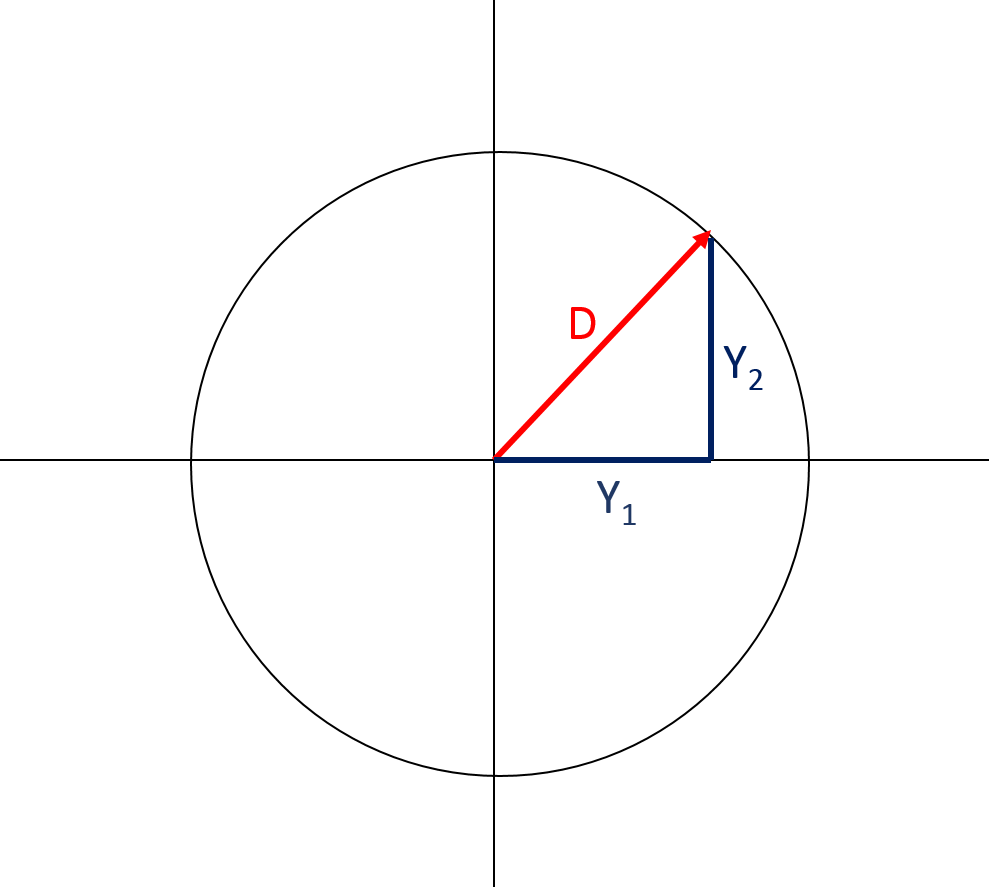
\includegraphics[width=3cm]{Picture1.png}
      \end{figure}
    \end{column}

    \begin{column}{5cm}
      \[ y_1 = D \cos \omega, \quad y_2 = D \sin \omega \quad \]
      \[ \text{where}\ D = \sqrt{-2 \log x_1}, \quad \omega = 2\pi x_2 \]
    \end{column}
  \end{columns}

  \bigskip
  
  \bigskip
  
  \[
    h^{-1}(x_1,x_2) = \begin{cases}
      x_1 = \exp{\left\{ -\frac{y_1^2 + y_2^2}{2} \right\}}       
      \\
      x_2 = \frac{1}{2\pi} \arctan \frac{y_2}{y_1}
    \end{cases}
  \]
  \[
  	|\text{Jacobian}| = \det \left(
  	  \begin{matrix}
  	    \frac{\partial x_1}{\partial y_1} & \frac{\partial x_1}{\partial y_2} \\
  	    \frac{\partial x_2}{\partial y_1} & \frac{\partial x_2}{\partial y_2} 
  	  \end{matrix}
  	\right) = 
  	\left[ 
  	  \frac{1}{\sqrt{2\pi}} \exp{\left(-\frac{y_1^2}{2}\right)}
  	\right]
  	\cdot
  	\left[
  	  \frac{1}{\sqrt{2\pi}} \exp{\left(-\frac{y_2^2}{2}\right)} 
  	\right]
  \]
  is the density of the bivariate standard normal distribution because it's the product of two univariate standard normal densities.
\end{frame}

\begin{frame}
  \frametitle{Polar method}
  \begin{enumerate}
    \item Let $U_1, U_2 \sim \mathcal{U}(0,1)$
    \item Define $V_i = 2U_i - 1$: $V_i \sim \mathcal{U}(-1,1)$
    \item Define $S = V_1^2 + V_2^2$
    \item If and only if $S \leq 1$, then define
      \[ Y = \sqrt{\frac{-2\ln{S}}{S}} \]
    \item \[
        \left( \begin{matrix} X_1 \\ X_2 \end{matrix} \right) = \left( \begin{matrix} V_1 Y \\ V_2 Y \end{matrix} \right)
        \quad \text{ and } \quad X_1,X_2\ \text{i.i.d.}\ \sim \mathcal{N}(0,1)
      \]
  \end{enumerate}  
\end{frame}

\begin{frame}
  \frametitle{Polar method}
  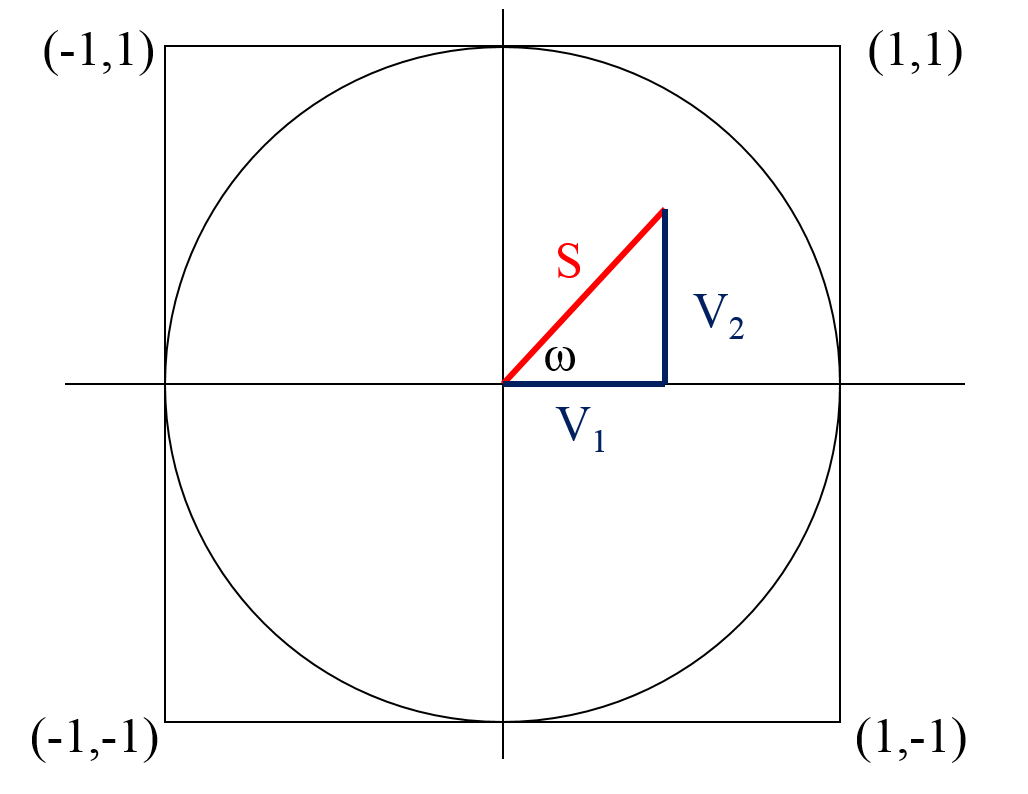
\includegraphics[width=\textwidth]{Picture2.png}
\end{frame}

\begin{frame}
  \frametitle{Correlated bivariate random variables}
  \[
    \mathbf{Z} = \left(\begin{matrix} z_1 \\ z_2 \end{matrix} \right), \quad z_1, z_2 \sim \mathcal{N}(0,1)
    \quad
    \mathbf{\mu} = \left(\begin{matrix} \mu_1 \\ \mu_2 \end{matrix} \right)
    \quad
    \Sigma = \left(\begin{matrix} \sigma_1^2 & \rho\sigma_1\sigma_2 \\ \rho\sigma_1\sigma_2 & \sigma_2^2 \end{matrix} \right)
  \]
  \begin{enumerate}
    \item Calculate the Cholesky decomposition $AA^T = \Sigma$
      \[
        \left(\begin{matrix} a & 0 \\ b & c \end{matrix} \right)
        \left(\begin{matrix} a & b \\ 0 & c \end{matrix} \right) =
        \left(\begin{matrix} a^2 & ab \\ ab & b^2 + c^2 \end{matrix} \right)
        = \left(\begin{matrix} \sigma_1^2 & \rho\sigma_1\sigma_2 \\ \rho\sigma_1\sigma_2 & \sigma_2^2 \end{matrix} \right)
      \] \[
        \rightarrow A = \left(\begin{matrix} \sigma_1 & 0 \\ \rho\sigma_2 & \sigma_2(1-\rho^2)^{\frac{1}{2}} \end{matrix} \right)
      \]
    \item Calculate $\mathbf{Z} \sim\mathcal{N}(0,\mathbb{I}_2)$
    \item $\mu + A\mathbf{Z} \sim \mathcal{N}(\mu,\Sigma)$ has the desired distribution.
      \[
        \left( \begin{matrix}X \\ Y \end{matrix} \right) = 
        \mu + %\left( \begin{matrix}\mu_1 \\ \mu_2 \end{matrix} \right) + 
          \left(\begin{matrix} \sigma_1 & 0 \\ \rho\sigma_2 & \sigma_2(1-\rho^2)^{\frac{1}{2}} \end{matrix} \right)
          \left(\begin{matrix} z_1 \\ z_2 \end{matrix} \right) =
        \mu + % \left( \begin{matrix}\mu_1 \\ \mu_2 \end{matrix} \right) + 
          \left(\begin{matrix} \sigma_1 z_1 \\ \rho\sigma_2z_1+\sigma_2(1-\rho^2)^\frac{1}{2}z_2 \end{matrix} \right)
      \]
  \end{enumerate}
\end{frame}

\begin{frame}
	\frametitle{Implementations - Linear Congruential Generator}
	\begin{columns}[t]
		\begin{column}{5cm}
      \inputminted[fontsize=\small,linenos]{matlab}{matlab/lcg.m}
		\end{column}
		\begin{column}{5cm}
      \inputminted[fontsize=\small,linenos,firstnumber=14]{matlab}{matlab/lcgstep.m}
		\end{column}
	\end{columns}
\end{frame}

\begin{frame}
	\frametitle{Implementations - Box-Muller method}
  \inputminted[fontsize=\small,linenos]{matlab}{matlab/boxmuller.m}
\end{frame}

\begin{frame}
	\frametitle{Implementations - Marsaglia polar algorithm}
  \inputminted[fontsize=\small,linenos]{matlab}{matlab/marsaglia.m}
\end{frame}

\begin{frame}
	\frametitle{Plots - Univariate methods}
	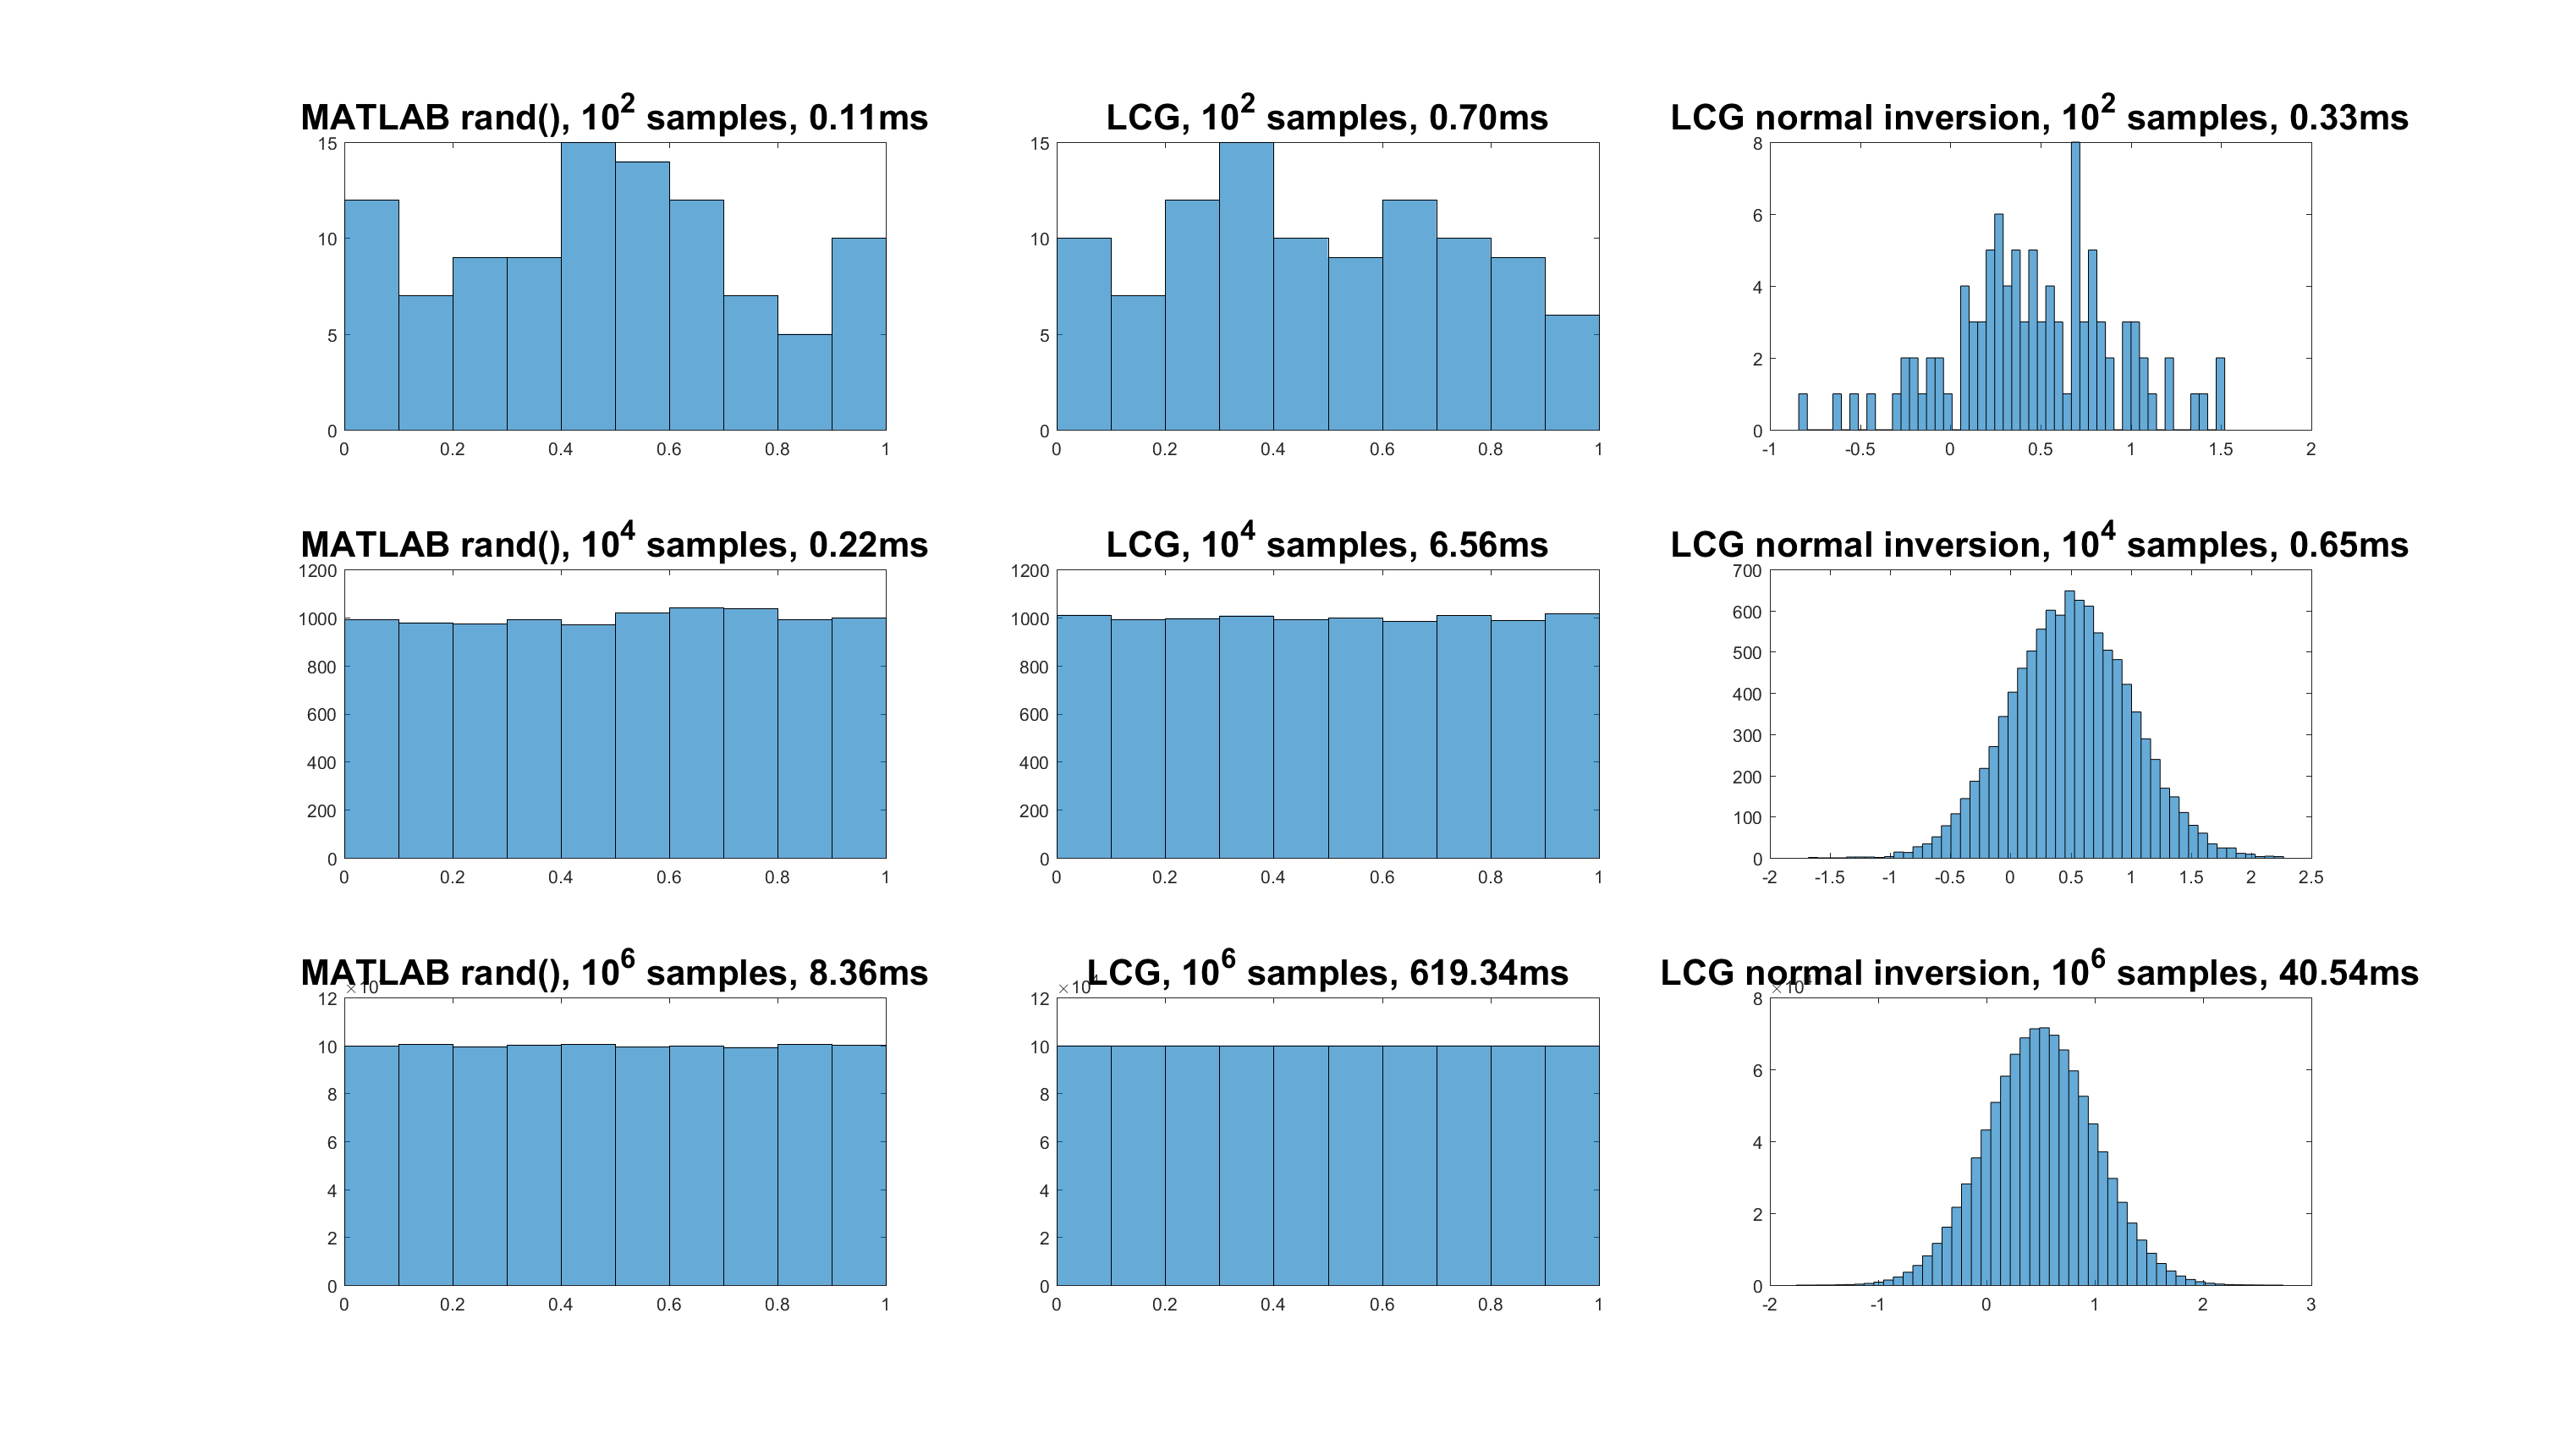
\includegraphics[width=\textwidth, trim=70mm 80mm 70mm 20mm]{../univariate.eps}
\end{frame}

\begin{frame}[fragile]
	\frametitle{Plots - Bivariate methods}
	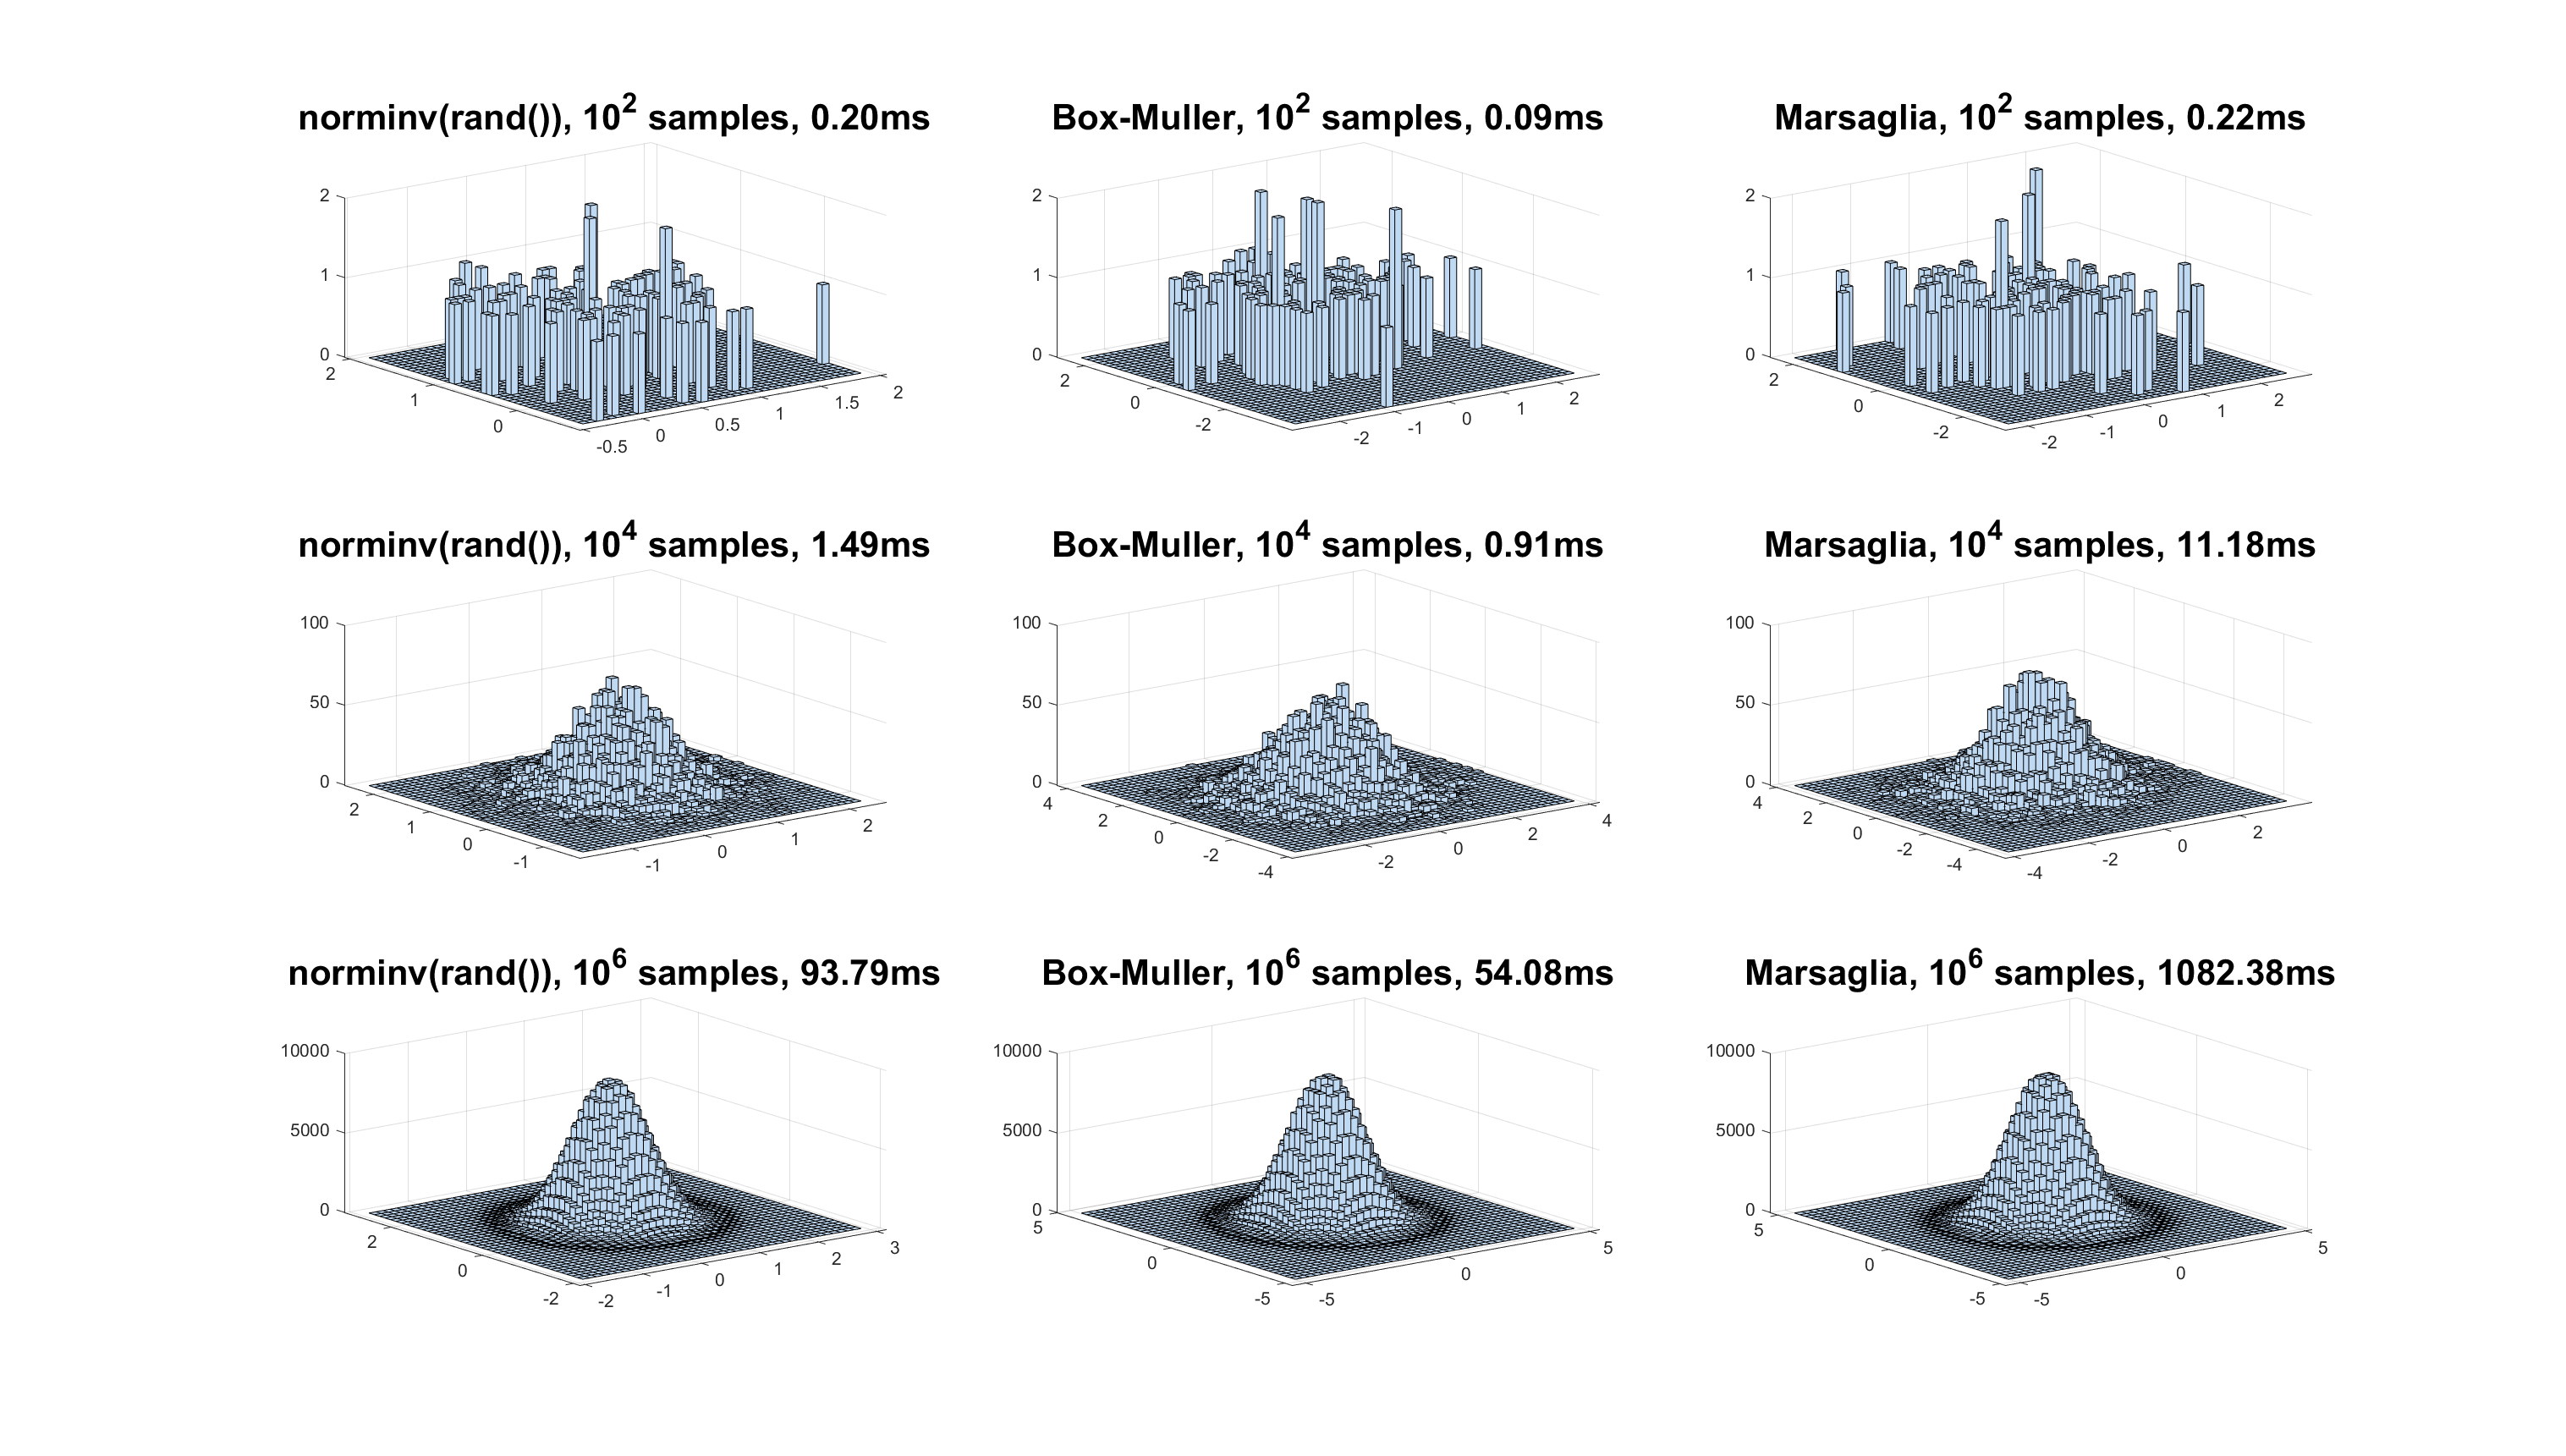
\includegraphics[width=\textwidth, trim=70mm 80mm 70mm 20mm]{../bivariate.eps}
\end{frame}

\end{document}
